\chapter{Avaliação e Resultados}\label{cap3}

O \autoref{cap2:treplica_reconfiguravel} apresentou três funcionalidades para expansão da
biblioteca Treplica:

\begin{enumerate}
  \item Protocolo para transferência de estado: criação de um mecanismo eficiente para
    transferência de estado entre réplicas.
  \item Réplicas leitoras: possibilidade da utilização de réplicas que não participam do
    processo de decisão de instâncias de consenso.
  \item Equalização de estado: proposta para novo componente de preenchimento de lacunas
    originadas por possíveis períodos de instabilidade da réplica e/ou falhas.
\end{enumerate}

Supomos duas hipóteses baseado-se nas alterações propostas 1 e 2. A alteração proposta
pelo item 3 não será validada por esse trabalho. Mantivemos a descrição dessa alteração
para enriquecimento do conteúdo e possível utilização em trabalhos futuros.

\begin{enumerate}
  \item Se possuirmos um mecanismo transferência eficiente, podemos recuperar o estado de
    uma réplica de forma mais eficiente que a aplicação do histórico de decreto do
    aglomerado. Lembrando que, toda réplica votante armazena em memória persistente
    qualquer alteração realizada no seu estado.
  \item Se possuirmos uma réplica que evite a reconfiguração total do sistema, ganharemos
    o poder de manobra necessário para expansão do aglomerado de acordo com a demanda de
    clientes.
\end{enumerate}

Para validar que a hipótese 1 e 2 podem aumentar o desempenho de um sistema que utiliza a
biblioteca Treplica, supomos uma carga de trabalho na qual uma parcela significativa das
requisições solicitadas para aplicação seja de leitura. Essa é uma suposição razoável para
a maioria das aplicações de Internet \cite{tpc02} e proporciona o cenário, que acreditamos
ser o mais adequado, para execução eficiente utilizando réplicas leitoras.

Começamos esse capítulo com a \autoref{sec:aplicacao}, apresentando os detalhes da
aplicação e as bibliotecas utilizadas para sua concepção. Em seguida, na
\autoref{sec:ambiente_experimental} descrevemos o ambiente experimental usado na execução
dos experimentos. As próximas duas seções \autoref{sec:experimento_tranferencia_estado} e
\autoref{sec:experimento_replicas_leitoras} apresentam respectivamente os experimentos de
transferência de estado e réplicas leitoras com seus respectivos cenários, resultados e
análise. Encerramos o capitulo com a \autoref{sec:conclusao} apresentando as considerações
finais.


\section{Aplicação}\label{sec:aplicacao}

Para fins experimentais, desenvolvemos então, visando a validação do conjunto de
experimentos, uma aplicação Web simples que mapeia uma cadeia de caracteres para um valor
numérico de 32 bits. Em outras palavras, criamos uma aplicação caracterizada como um mapa
que disponibiliza dois serviços aos clientes remotos através de uma interface HTTP:

\begin{enumerate}
  \item Operação GET \verb|/replicated-map/map/key/<chave>|
  \item Operação PUT \verb|/replicated-map/map/key/<chave>/value/<valor>|
\end{enumerate}

A operação GET é uma operação de leitura, sua função proporciona ao cliente buscar o valor
armazenado em uma determinada chave. Definimos que uma operação bem-sucedida no método GET
retorna o código de status HTTP 200 e um JSON com o valor da chave requisitada
\verb|{"value":"<valor>"}|. Por outro lado, o método PUT defini operações de escrita, ele
é responsável por armazenar um valor em uma determinada chave. Definimos que uma operação
de escrita sem falhas não possui corpo de retorno, o método retorna apenas o código de
status HTTP 201.

Utilizamos a linguagem Scala\footnote{\url{http://www.scala-lang.org}} para criação da
aplicação, sendo que o estado da aplicação é gerenciado pela biblioteca Treplica que atua
como um \emph{middleware} de replicação ativa, conforme ilustra a figura
\autoref{fig:treplica_como_middleware}. Treplica é uma biblioteca Java e mostrou boa
interoperabilidade com a aplicação. Não relatamos nenhum problema oriundo da utilização de
bibliotecas Java com a linguagem Scala.

\begin{figure}[ht]
  \centering
  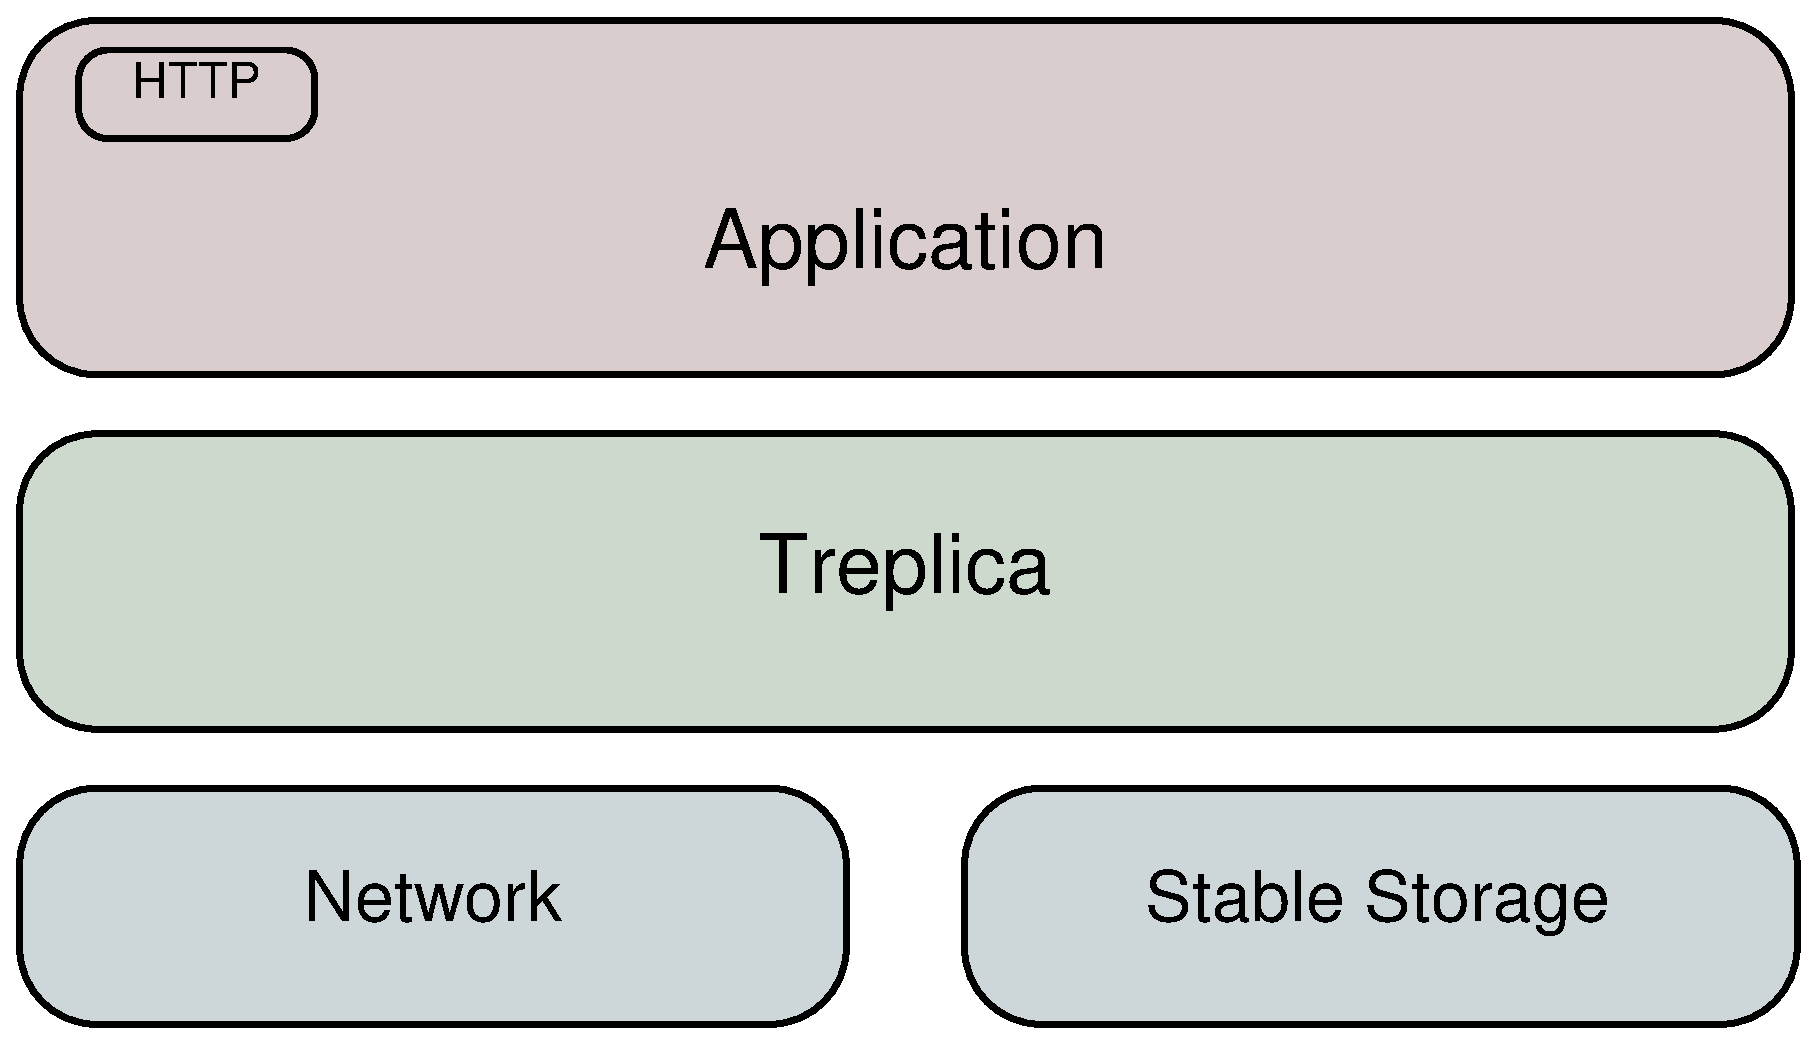
\includegraphics[width=12cm]{conteudo/capitulos/figuras/block-treplica.eps}
  \caption{Treplica como \emph{middleware} de replicação ativa}
  \label{fig:treplica_como_middleware}
\end{figure}

Apesar da simplicidade encontrada na aplicação de teste, ela é executada em um aglomerado
de máquinas e oferece pra seus clientes, a garantia de que toda operação de escrita será
replicada para outras instâncias de forma ativa. Com base nessa propriedade, garantimos a
elegibilidade dessa aplicação para execução de experimentos no modelo computacional
utilizando replicação ativa.

Cada uma das réplicas instanciadas possui seu próprio estado e podem assumir diferentes
graus de persistência para dos dados em memória, definido-as como réplicas votantes ou
réplicas leitoras:

\begin{itemize}
  \item Réplica votante: utiliza memória persistente, premissa do algoritmo Paxos para
    garantia de correção no modelo computacional falha-e-recuperação.
  \item Réplica leitora: utiliza memória volátil.
\end{itemize}

\subsection{Dependências}

A \autoref{tab:dependencias} lista as bibliotecas dependentes, com a respectiva versão
utilizada, utilizadas para compilação e execução da aplicação. A tabela lista também a
responsabilidade que a biblioteca exerce no projeto.

\begin{table}[htb]
\IBGEtab{
  \caption{Tabela de dependência de bibliotecas}
  \label{tab:dependencias}
}{
  \begin{tabular}{ccc}
  \toprule
    Biblioteca & Versão & Responsabilidade \\
  \midrule \midrule
    treplica & 0.3.2 & \emph{midleware} de replicação ativa \\
  \midrule
    vraptor & 3.5.1 & controlador MVC \\
  \bottomrule
\end{tabular}
}{
  \fonte{Produzido pelos autores.}
  \nota{Vraptor: \url{http://vraptor3.vraptor.org}}
  \nota{Model-View-Controller, é um padrão de projeto de software que separa a
  representação da informação da iteração do usuário \cite{alguem}}
}
\end{table}

\section{Descrição do Ambiente Experimental}\label{sec:ambiente_experimental}

Os experimentos foram realizados em um aglomerado com 16 nós, interligados através de um
\emph{switch} Ethernet de 1 Gbps. Cada nó possui a seguinte capacidade de processamento:

\begin{itemize}
  \item 1 processador Xeon E5620 (2.4 GHz, 6 \emph{threads});
  \item 12 GB de memória RAM;
  \item 500 GB de armazenamento local (disco 7200 rpm);
  \item Plataforma de 64 bits;
\end{itemize}

Os nós utilizam o sistema operacional GNU/Linux Debian 6.0. A \autoref{tab:aplicativos}
lista os aplicativos e suas respectivas versões que foram utilizados para execução dos
experimentos.

\begin{table}[htb]
\IBGEtab{
  \caption{Tabela de aplicativos utilizados nos experimentos}
  \label{tab:dependencias}
}{
  \begin{tabular}{ccc}
  \toprule
    Aplicativo & Versão & Descrição \\
  \midrule \midrule
    JVM & HotSpot 64-Bit 1.7.0\_45 & Máquina Virtual Java \\
  \midrule
    Apache Tomcat & 7.0.32 & \emph{Servlet container} \\
  \midrule
    HAProxy & 1.5-dev19 & \emph{HTTP Load balancer} \\
  \bottomrule
\end{tabular}
}{
  \fonte{Produzido pelos autores.}
  \nota{Apache Tomcat: \url{http://tomcat.apache.org}}
  \nota{HAProxy: \url{http://www.haproxy.org}}
}
\end{table}

O conjunto de réplicas é gerenciado por um servidor balanceador de carga configurado com
HAProxy, usado para melhorar o desempenho de serviços Web distribuindo requisições entre
vários servidores. Todas as requisições dos clientes passam pelo HAProxy, configurado para
receber e rotear as requisições para as réplicas ativas, usando um algoritmo de
revezamento circular (\emph{round-robin}), como ilustrado na \autoref{fig:setup}. Nessa
configuração os processos clientes não compartilham recursos com os processos da
aplicação, ou seja, ou a instância executa processos clientes ou executa processos da
aplicação.

\begin{figure}[ht]
  \centering
  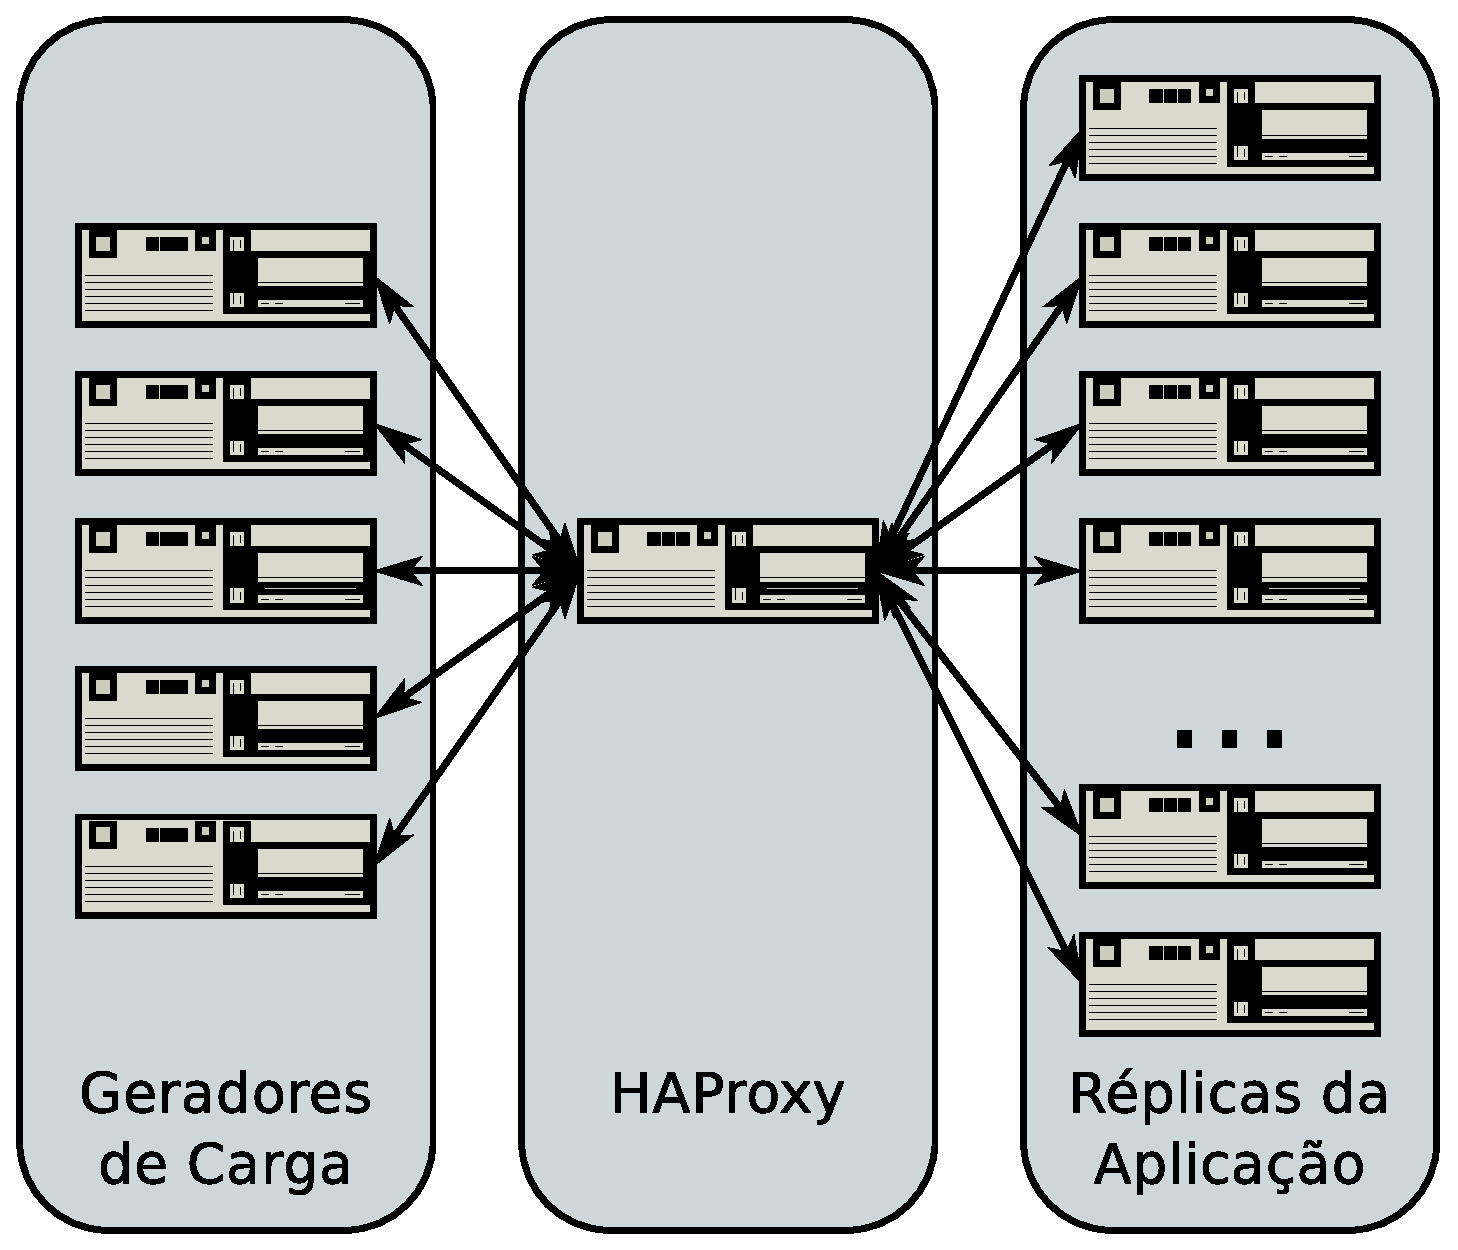
\includegraphics[width=7cm]{conteudo/capitulos/figuras/experimental-setup.dia.eps}
  \caption{Configuração experimental}
  \label{fig:setup}
\end{figure}

\subsection{Carga}

O programa de teste tem por objetivo produzir a carga de trabalho requirida pelos
experimentos e coletar medidas de vazão do ponto de vista do cliente. Sendo assim, o
programa de teste, em cada instância, registra em \emph{log} o \emph{timestamp} de início
e fim de cada atividade para que seja possível o computar a vazão alcançada pela
aplicação.

Para geração da carga de trabalho utilizamos processos Java que executam requisições de
leitura (requisições para o método HTTP GET) e escrita (requisições para o método HTTP
PUT) respeitando um percentual configurável para realização de cada operação. Para todos
os experimentos dedicamos 5 máquinas para atuarem como clientes, sendo que cada uma
executa 1000 requisições/segundo, variando (sem garantia de ordem) entre requisições de
leitura e escrita.

Do ponto de vista da aplicação, requisições de leitura serão atendidas localmente por uma
das réplicas, enquanto uma requisição de escrita será transformada em uma proposta e
submetida a uma rodada de consenso entre as réplicas votantes. Avaliando-se o custo de
cada tipo de requisição, podemos afirmar que requisições de escritas são mais caras porque
envolvem mais trocas de mensagens que requisições de leitura.

Cada teste identificará o percentual de execução de cada operação. A partir dessa
configuração, foi gerado uma carga total para aplicação de 5000 requisições/segundo. O
tempo total de execução de cada experimento foi de 180 segundos. Para a análise
consideramos um intervalo de 140 segundos que é resultado do descarte dos 20 segundos
iniciais e finais. O desempenho foi medido através da quantidade de requisições HTTP
atendidas e o tempo de resposta.


\section{Experimento Transferência de Estado}\label{sec:experimento_tranferencia_estado}

Esse experimento está fundamentada na possível disparidade de estado existente entre
réplicas. Para construção desse cenário supomos um aglomerado com cinco réplicas, todas
previamente configuradas com a aplicação de teste. Nosso objetivo é a geração da
divergência do estado replicado em uma das réplicas, para alcançar esse objetivo iniciamos
quatro réplicas simultaneamente e postergamos a inicialização de uma das réplicas.
Definimos então dois instantes no tempo:

\begin{itemize}
  \item $t1$ início da execução das requisições dos clientes;
  \item $t2$ inicialização da aplicação na última réplica, $t2$ acontece exatamente 180
    segundos após $t1$.
\end{itemize}

Nessa configuração, o momento $t1$ possui quatro réplicas prontas para atender as
requisições dos clientes. Do ponto de vista do algoritmo Paxos, ainda está faltando uma
réplica, pois devido a característica estática da definição do total de réplicas, essa
propriedade foi previamente definida como cinco. Nesse cenário a formação de quórum para
definição de consenso só não é legitima quando: (1) No intervalo entre $t1$ e $t2$ duas
réplicas falham; (2) Após $t2$, três máquinas falham.

Analisando as restrições que definem o estado da aplicação sem progresso, podemos afirmar
que a inclusão de uma nova réplica no momento $t2$ aumenta a tolerância a falhas da
aplicação. No entanto essa afirmação é verdadeira, se e somente se, a réplica adicionada
em $t2$ é uma réplica votante. A tolerância a falhas é uma propriedade baseada nas
réplicas votantes, que não se altera em caso de adição de réplicas leitoras.

Nessa versão de Treplica, o mecanismo de transferência de estado é exclusivo das réplicas
leitoras, abriremos mão da propriedade de tolerância a falhas para adicionarmos, em $t2$,
uma réplicas leitora para medir o impacto que o protocolo de transferência de estado
causa na aplicação. Para criação de uma base de comparação, o mesmo teste foi executado
adicionando uma réplica votante, sem o mecanismo de transferência de estado. Nesse caso, a
equalização do estado (preenchimento da lacuna) é realizado pelo mecanismo de
retransmissão de instância de consenso existente em Treplica.


\fbox{\begin{minipage}
  Lorem ipsum dolor sit amet, his at eruditi civibus. Mei mucius labores delicata ut,
  fuisset qualisque ut sea, pro invidunt theophrastus ei. Alterum accusam usu ex, id duo
  verear sapientem. Pro velit minim oblique et, diam meis ea usu. Per at tantas deserunt,
  lorem laboramus ca vel. Lobortis concludaturque mel ex, at liber viderer delicatissimi
  eos, eu vel altera sadipscing. Ad cum unum posse urbanitas. Vim idque hendrerit cu, homero
  bonorum omittam cu pro. Idque doming eu his, his te alias hinc.
\end{minipage}}

Cenários, carga, servidores

Resultados

Análise

\section{Experimento Elástico}\label{sec:experimento_replicas_leitoras}

Cenários, carga, servidores

Resultados

Análise


Descrever a proposta e sua implementação.

\section{Conclusão}\label{sec:conclusao}

